% !TeX program = xelatex
% Overleaf 编译器请选择 XeLaTeX。将本文件与四张 PNG 图片放在同一目录即可编译。
\documentclass[UTF8,a4paper,12pt]{ctexart}

\usepackage[left=2.5cm,right=2.5cm,top=2.6cm,bottom=2.6cm]{geometry}
\usepackage{amsmath,amssymb}
\usepackage{booktabs,tabularx,array,longtable,multirow}
\usepackage{enumitem}
\usepackage{xcolor}
\usepackage{hyperref}
\usepackage{float}
\usepackage{caption}
\usepackage{graphicx}
\usepackage{setspace}

\hypersetup{
  colorlinks=true,
  linkcolor=blue!55!black,
  citecolor=blue!55!black,
  urlcolor=blue!65!black,
  pdftitle={基于 ReChorus 的 SimGCL 推荐算法复现实验},
  pdfauthor={课程实验小组}
}
\setlength{\parindent}{2em}
\setlength{\parskip}{0.25em}
\setlength{\emergencystretch}{2em}
\setlist[itemize]{leftmargin=2.2em,itemsep=0.2em,topsep=0.3em}
\setlist[enumerate]{leftmargin=2.4em,itemsep=0.2em,topsep=0.3em}
\renewcommand{\arraystretch}{1.18}
\captionsetup{font=small,labelfont=bf}

\title{\bfseries 基于 ReChorus 的 SimGCL 推荐算法复现实验\\
\large 图对比学习方法实现、完整数据对比与可复现性审计}
\author{
  课程：机器学习 \quad 小组：第 43 组 \\[0.5em]
  组员1：\underline{\makebox[3.5cm][c]{鲁越}} \quad 学号：\underline{\makebox[3.5cm][c]{24334089}} \\[0.5em]
  组员2：\underline{\makebox[3.5cm][c]{何天佑}} \quad 学号：\underline{\makebox[3.5cm][c]{24334040}}
}

\begin{document}
\pagestyle{plain}

\maketitle

\begin{abstract}
\normalsize
\setstretch{1.35}
本文在轻量级推荐算法框架 ReChorus 中复现了 SIGIR 2022 图对比推荐模型 SimGCL，并选择同属 General Recommender 的 BPRMF 与 LightGCN 作为基线，在 Amazon Grocery 和 MovieLens-1M 两个框架数据集上进行统一比较。实现包含 LightGCN 图传播、逐层同超象限随机噪声增强、用户侧与物品侧 InfoNCE 以及 BPR 联合优化，并消除了上游 LightGCN 对 CUDA 的硬编码依赖。实验先在可重复的 CPU 子集上验证实现并研究对比损失权重，随后在完整数据上采用 64 维嵌入、3 层传播、batch size 2048、最多 200 轮和基于验证集 NDCG@20 的早停策略完成 6 组对比。完整 Grocery 数据上，SimGCL 的 NDCG@20 达到 0.2042，高于 LightGCN 的 0.1750；但其 HR@20 为 0.3896，低于 LightGCN 的 0.4186。MovieLens-1M 上，LightGCN 整体最优，而固定 $\lambda=0.2$ 的 SimGCL 未取得优势。

\noindent\textbf{关键词：}推荐系统；图对比学习；SimGCL；LightGCN；ReChorus；可复现性
\end{abstract}

\tableofcontents
\clearpage

\section{实验背景与任务要求}

推荐系统需要从稀疏的用户--物品交互中学习偏好表示。矩阵分解可以直接建模用户和物品的潜在向量，图协同过滤进一步利用用户--物品二部图上的高阶邻居信息，而图对比学习通过构造多个相关视图，为表示空间加入自监督约束。传统图对比推荐方法通常依赖节点删除、边删除或随机游走等结构增强，但这些操作需要重复构造图，并可能破坏对推荐有用的连接。SimGCL~\cite{simgcl} 提出直接在图传播表示上加入受约束噪声，用更简单的方式获得两个对比视图。

本实验依据课程文档完成以下任务：

\begin{enumerate}
  \item 使用指定的 ReChorus 框架复现 SimGCL；
  \item 选择不少于两个同类别算法作为基线；
  \item 在不少于两个框架数据集上进行统一实验；
  \item 在报告中说明技术原理、具体实现、创新点、实验结果和分析；
  \item 提供可复现代码、README、训练日志、模型检查点及汇总结果。
\end{enumerate}

本实验选择 BPRMF 与 LightGCN 两个 General Recommender 作为基线。三种模型共享相同的数据文件、训练负采样、候选集合和评价函数，从而把比较差异尽量限制在模型本身。项目代码位于随报告提交的 \path{ReChorus} 目录。GitHub 仓库地址为 \url{https://github.com/lipengpai/-ReChorus-SimGCL-.git}。

\section{相关技术原理}

\subsection{ReChorus 框架}

ReChorus 将推荐实验拆分为 Reader、Model 和 Runner 三类核心模块~\cite{rechorus}。Reader 统一读取训练、验证和测试文件，统计用户数、物品数及用户历史；Model 定义参数、前向传播、损失函数和批数据格式；Runner 负责负采样、优化、验证、早停、检查点保存与指标计算。这种分离方式使新增模型通常只需实现一个模型文件，同时复用统一的数据与评价逻辑。

本项目把 SimGCL 实现为 \path{src/models/general/SimGCL.py}，继承 ReChorus 的 \texttt{GeneralModel}，并使用 \texttt{BaseReader} 与 \texttt{BaseRunner}。因此 BPRMF、LightGCN 和 SimGCL 在同一候选排序协议下计算 HR 与 NDCG。

\begin{figure}[H]
  \centering
  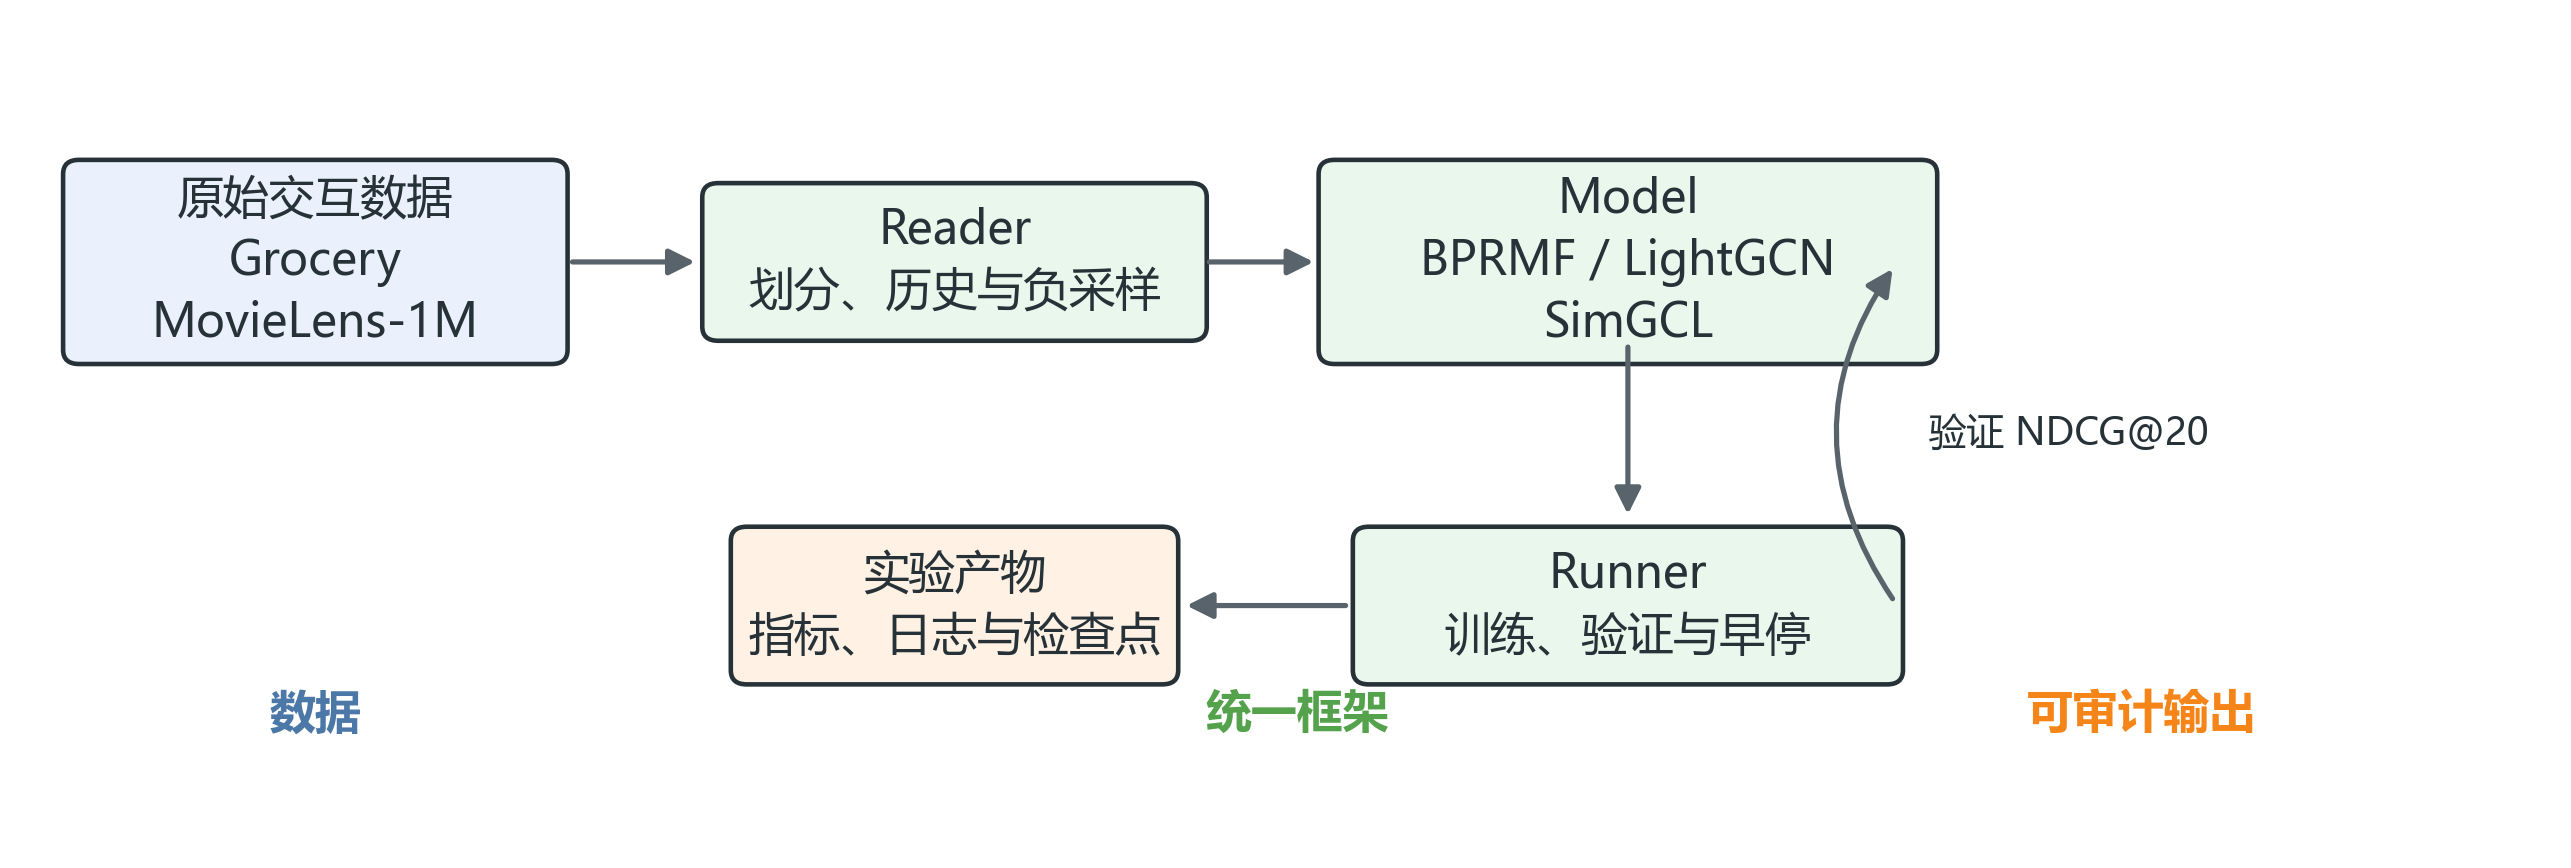
\includegraphics[width=0.96\textwidth]{fig1_rechorus_pipeline.png}
  \caption{基于 ReChorus 的统一实验流程。三种模型共享 Reader、Runner 与评价协议。}
  \label{fig:rechorus-pipeline}
\end{figure}

\subsection{BPRMF 与 LightGCN}

BPRMF 为每个用户 $u$ 和物品 $i$ 学习向量 $\mathbf e_u,\mathbf e_i$，预测分数为内积
\begin{equation}
  \hat y_{ui}=\mathbf e_u^{\top}\mathbf e_i.
\end{equation}
对正物品 $i$ 和负物品 $j$，BPR 损失为
\begin{equation}
  \mathcal L_{\mathrm{BPR}}
  =-\sum_{(u,i,j)}\log \sigma(\hat y_{ui}-\hat y_{uj}).
\end{equation}
它直接优化正物品相对负物品的排序关系，是本实验最基础的协同过滤基线~\cite{bpr}。

LightGCN~\cite{lightgcn} 将交互数据表示为无向二部图。设 $\widetilde{\mathbf A}=\mathbf D^{-1/2}\mathbf A\mathbf D^{-1/2}$ 为对称归一化邻接矩阵，第 $l$ 层传播为
\begin{equation}
  \mathbf E^{(l)}=\widetilde{\mathbf A}\mathbf E^{(l-1)}.
\end{equation}
LightGCN 删除了传统 GCN 中的特征变换与非线性激活，只保留邻居聚合，最终表示为各层嵌入的平均。与 BPRMF 相比，它能显式利用多跳协同关系。

\subsection{SimGCL}

SimGCL 的核心判断是：图对比学习带来的主要收益来自 InfoNCE 对表示均匀性的调节，而昂贵的结构增强并非必要。模型仍使用 LightGCN 作为编码器，但在每一层传播后加入随机扰动：
\begin{align}
  \bar{\mathbf E}^{(l)} &= \widetilde{\mathbf A}\mathbf E^{(l-1)},\\
  \mathbf E^{(l)} &= \bar{\mathbf E}^{(l)}+\boldsymbol\Delta^{(l)},\\
  \boldsymbol\Delta^{(l)}
  &=\epsilon\,\operatorname{normalize}(\mathbf R^{(l)})
  \odot\operatorname{sign}(\bar{\mathbf E}^{(l)}),
  \quad \mathbf R^{(l)}\sim U(0,1).
\end{align}
其中 $\epsilon$ 控制噪声的 L2 长度。乘以当前表示的符号后，噪声与原表示处于同一超象限，从而在产生差异的同时避免过大的语义偏移。两次独立噪声传播得到视图 $\mathbf z'$ 与 $\mathbf z''$。按照论文设置，SimGCL 聚合第 1 至第 $L$ 层，跳过第 0 层输入嵌入：
\begin{equation}
  \mathbf z=\frac{1}{L}\sum_{l=1}^{L}\mathbf E^{(l)}.
\end{equation}

对批内同一节点构成正对，其余节点作为负例。归一化表示上的 InfoNCE 为
\begin{equation}
  \mathcal L_{\mathrm{CL}}
  =-\sum_{i\in\mathcal B}
  \log\frac{\exp(\mathbf z_i'^{\top}\mathbf z_i''/\tau)}
  {\sum_{j\in\mathcal B}\exp(\mathbf z_i'^{\top}\mathbf z_j''/\tau)},
\end{equation}
其中 $\tau$ 为温度。实现分别计算用户侧和正物品侧损失，批内重复 ID 只保留一次，联合目标为
\begin{equation}
  \mathcal L
  =\mathcal L_{\mathrm{BPR}}
  +\lambda\left(\mathcal L_{\mathrm{CL}}^{u}
  +\mathcal L_{\mathrm{CL}}^{i}\right)
  +\beta\lVert\Theta\rVert_2^2.
\end{equation}

\section{系统实现}

\subsection{模型接入}

SimGCL 的实现包含以下关键步骤：

\begin{itemize}
  \item 使用训练集点击集合构造用户--物品二部图，并生成稀疏对称归一化邻接矩阵；
  \item 将邻接矩阵注册为 PyTorch buffer，使模型执行 \texttt{to(device)} 时图结构与参数同步迁移；
  \item 推荐分支使用无噪声传播，训练阶段额外执行两次独立噪声传播；
  \item 对用户 ID 和正物品 ID 分别去重，避免同一节点在批内被错误地当作自身负例；
  \item 使用交叉熵的数值稳定形式实现平均 InfoNCE；
  \item 单独保存 \texttt{pos\_item\_id}，避免 Runner 随机打乱候选位置后丢失真实正物品。
\end{itemize}

上游 LightGCN 的稀疏邻接矩阵原先被无条件移动到 CUDA，CPU 环境会直接失败。本项目将其改为模块 buffer，从而同时支持 CPU 和 GPU。

\subsection{数据预处理}

MovieLens-1M 预处理脚本读取 \texttt{ratings.dat}，保留评分不低于 4 的正反馈，执行正反馈 5-core 过滤，加入小时、星期和时间段上下文，再按全局日期约 8:1:1 划分训练、验证和测试。只保留训练中出现过的验证/测试用户与物品，并为每个验证/测试正例无放回采样 99 个该用户从未交互的物品。脚本固定随机种子并输出 ID 映射和统计 JSON。

需要明确区分实验协议：2022 年 ReChorus 论文采用逐用户留一法，而本项目遵循当前 ReChorus 2.0 随附的 MovieLens Top-K notebook；SimGCL 原论文则采用 7:1:2 划分和全物品排序。因此本文关注同一框架内部的公平比较，不直接复刻原论文表格的绝对数值。

\subsection{中断恢复与可审计性}

完整数据实验采用一组模型一次调用的分段方式。运行器会跳过已有最终测试行的组合，并累计规范日志中的历史训练时间，使 10 小时上限跨进程启动生效。每个完整轮次还保存最后模型、Adam 优化器、验证历史以及 Python、NumPy、PyTorch 随机状态；若发生异常中断，可从上一完整轮继续，而不是只加载最佳模型权重。

训练日志、最佳检查点、完整轮状态、汇总 CSV 与状态 JSON 分目录保存。曾经发生过人工暂停的旧日志和模型保存在 \path{results_full_cpu/interrupted}，不会覆盖最终连续运行结果。

\section{实验设计}

\subsection{数据集}

\begin{table}[H]
  \centering
  \caption{完整数据集统计}
  \label{tab:full-data}
  \begin{tabular}{lrrrrr}
    \toprule
    数据集 & 用户数 & 物品数 & 训练交互 & 验证交互 & 测试交互\\
    \midrule
    Grocery & 14,681 & 8,713 & 121,892 & 14,681 & 14,681\\
    MovieLens-1M & 6,032 & 3,125 & 568,731 & 2,589 & 2,877\\
    \bottomrule
  \end{tabular}
\end{table}

为了先验证代码正确性并控制试错成本，还构造了两个确定性 CPU 子集。

\begin{table}[H]
  \centering
  \caption{资源受限子集统计}
  \label{tab:pilot-data}
  \begin{tabular}{lrrrrr}
    \toprule
    数据集 & 用户数 & 物品数 & 训练交互 & 验证交互 & 测试交互\\
    \midrule
    Grocery\_Pilot & 500 & 2,978 & 4,211 & 500 & 500\\
    ML\_1M\_Pilot & 100 & 2,645 & 26,745 & 1,226 & 772\\
    \bottomrule
  \end{tabular}
\end{table}

\subsection{参数设置}

\begin{table}[H]
  \centering
  \caption{主要实验参数}
  \label{tab:settings}
  \begin{tabularx}{\textwidth}{lXX}
    \toprule
    设置 & 资源受限子集 & 完整数据\\
    \midrule
    随机种子 & 2026 & 2026\\
    嵌入维度 & 32 & 64\\
    图传播层数 & 2 & 3\\
    batch size & 1024 & 2048\\
    优化器与学习率 & Adam，0.001 & Adam，0.001\\
    L2 系数 & $10^{-4}$ & $10^{-4}$\\
    最大轮次 & 10 & 200\\
    早停 patience & 3 & 5；早期两组历史基线为 10\\
    SimGCL & $\tau=0.2,\epsilon=0.1$ & $\lambda=0.2,\tau=0.2,\epsilon=0.1$\\
    评价 & 1 正例 + 99 负例 & 1 正例 + 99 负例\\
    \bottomrule
  \end{tabularx}
\end{table}

完整数据中 Grocery 的 BPRMF 与 LightGCN 在修改早停要求前已经使用 patience=10 完成。日志表明两者最佳轮次分别为 23 和 25，之后未再改善；因此保留其最佳检查点。其余完整实验统一使用 patience=5。

子集调参只依据验证集 NDCG@20，搜索 $\lambda\in\{0.01,0.05\}$ 与 \texttt{include\_ego}$\in\{0,1\}$，不读取测试指标进行选参。完整数据使用统一参考配置 $\lambda=0.2$，目的是在有限 CPU 预算下进行受控对比。SimGCL 原论文并不存在适用于所有数据集的固定最优 $\lambda$，因此本文不把该设置称为论文最优参数。

\subsection{评价指标}

每个评价列表只有一个正例，因此 HR@K 与 Recall@K 数值等价。设正例排序为 $r$，则
\begin{align}
  \mathrm{HR@K} &= \mathbb I(r\le K),\\
  \mathrm{NDCG@K} &= \frac{\mathbb I(r\le K)}{\log_2(r+1)}.
\end{align}
本文报告 HR@10、NDCG@10、HR@20 和 NDCG@20，并以验证集 NDCG@20 选择最佳检查点与执行早停。

\section{实验过程}

实验按以下顺序进行：

\begin{enumerate}
  \item 阅读 SimGCL 与 ReChorus 论文，确定模型公式、框架接口和评价方式；
  \item 实现 SimGCL，修复 LightGCN 的 CPU 兼容问题；
  \item 编写 MovieLens 确定性预处理与子集构造脚本；
  \item 在两个子集上运行 BPRMF、LightGCN 和 SimGCL，验证前向、反向与结果汇总；
  \item 仅使用验证集完成小网格调参；
  \item 在两个完整数据集上依次运行三种模型，并保存日志与检查点；
  \item 对 MovieLens SimGCL 的人工中断进行审计。发现旧检查点未保存 Adam 状态后，废弃该续跑结果，并从随机种子 2026 重新连续运行；
  \item 独立加载最终检查点进行只评估复算，并执行全部自动测试。
\end{enumerate}

\begin{figure}[H]
  \centering
  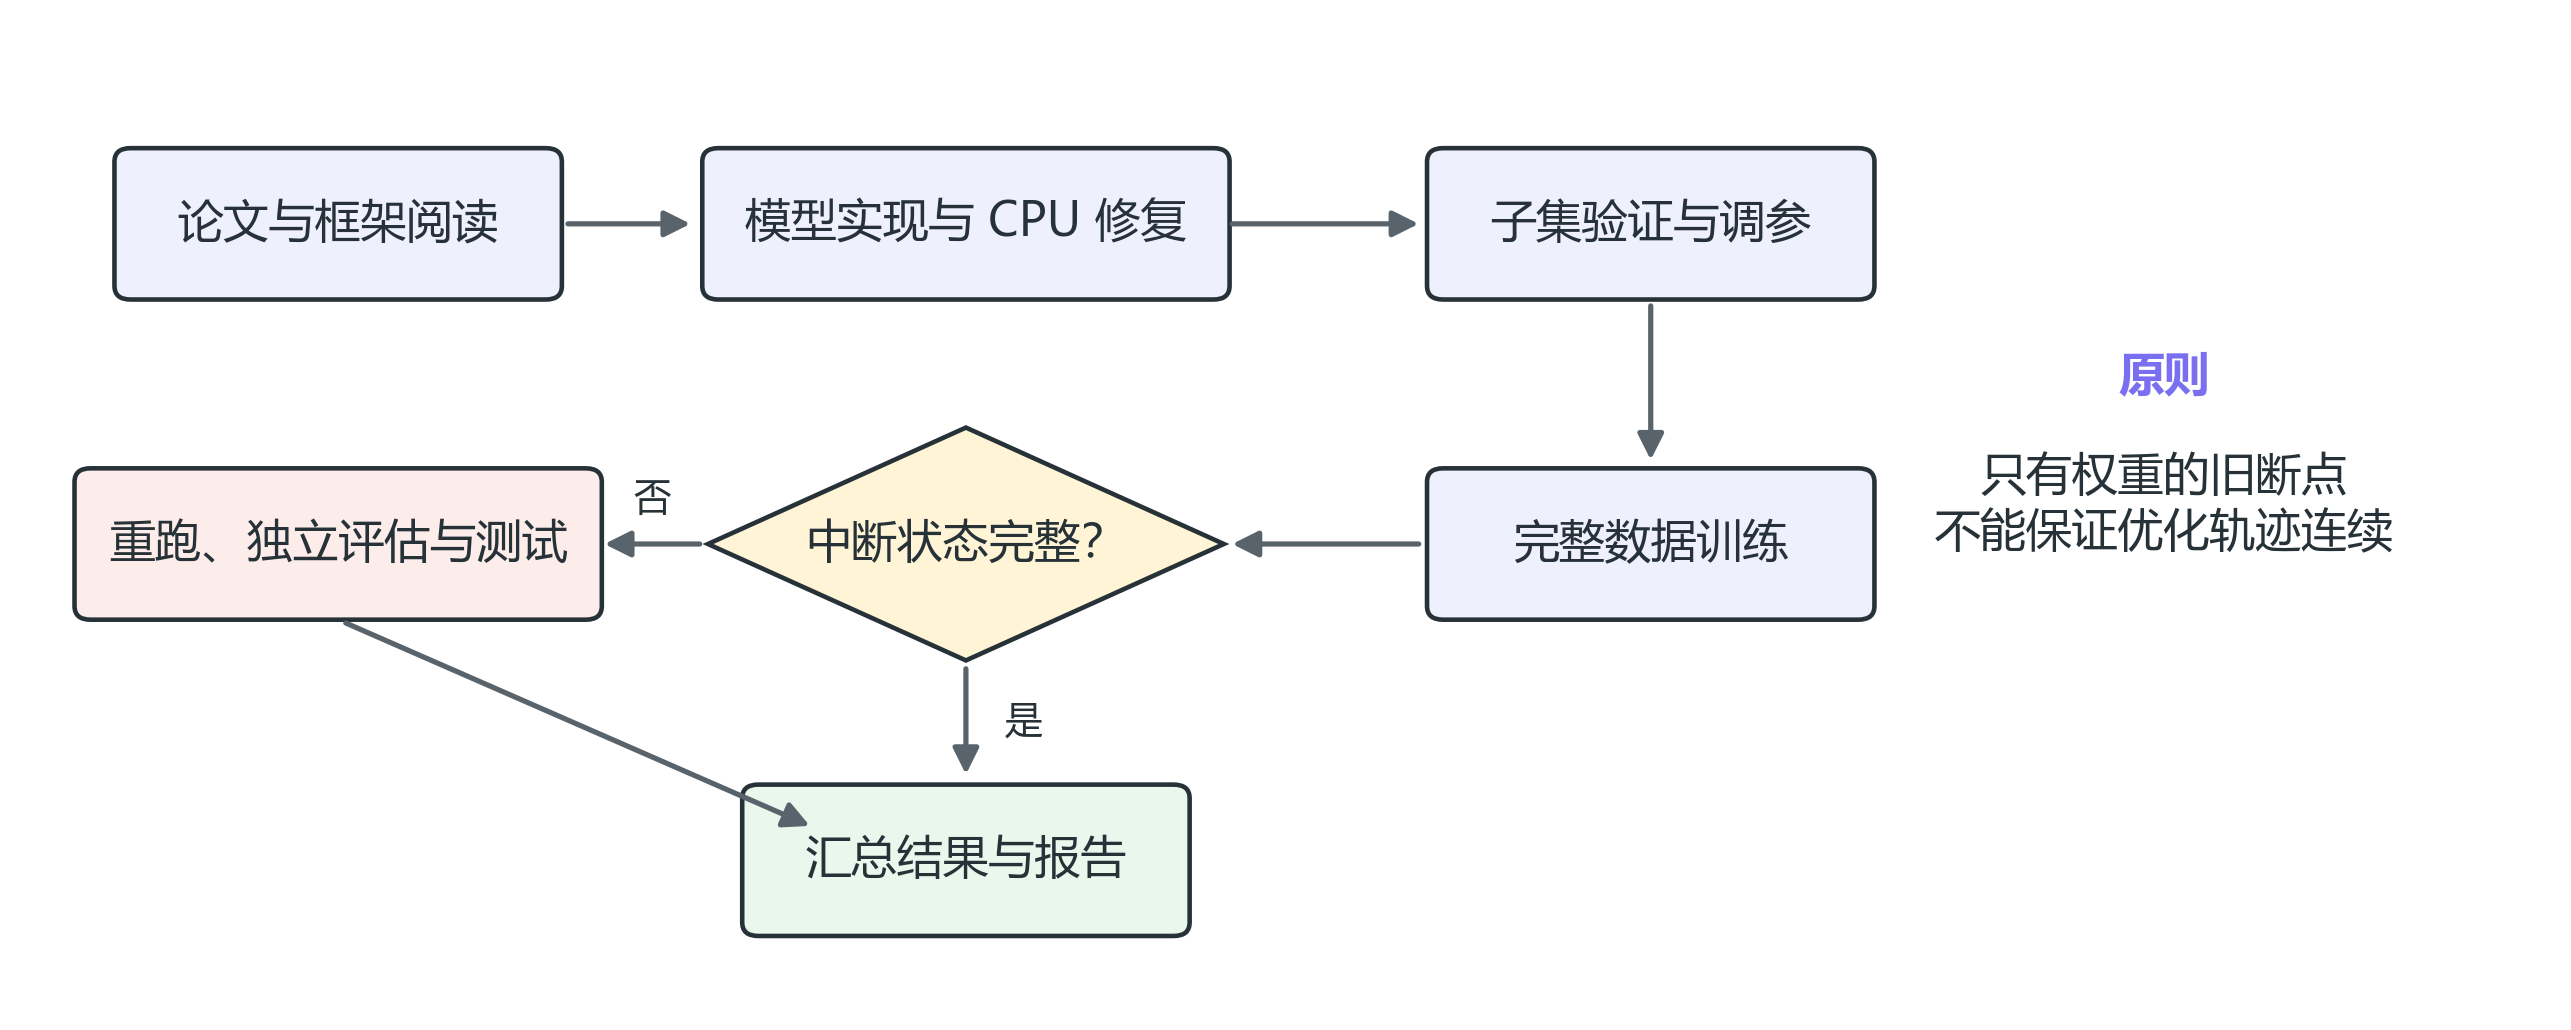
\includegraphics[width=0.96\textwidth]{fig2_experiment_process.png}
  \caption{实验执行与中断审计流程。旧断点缺少优化器状态时，不将续跑结果作为最终结果。}
  \label{fig:experiment-process}
\end{figure}

连续重跑的 MovieLens SimGCL 在第 1--6 轮上的验证 NDCG@20 依次为 0.2059、0.1975、0.1957、0.1957、0.1908 和 0.1939。第 1 轮为最佳，之后连续 5 轮未提升，因此第 6 轮结束时触发早停。连续运行与旧的权重续跑在第 2 轮损失上已经出现差异，说明重新运行是必要的。

\begin{figure}[H]
  \centering
  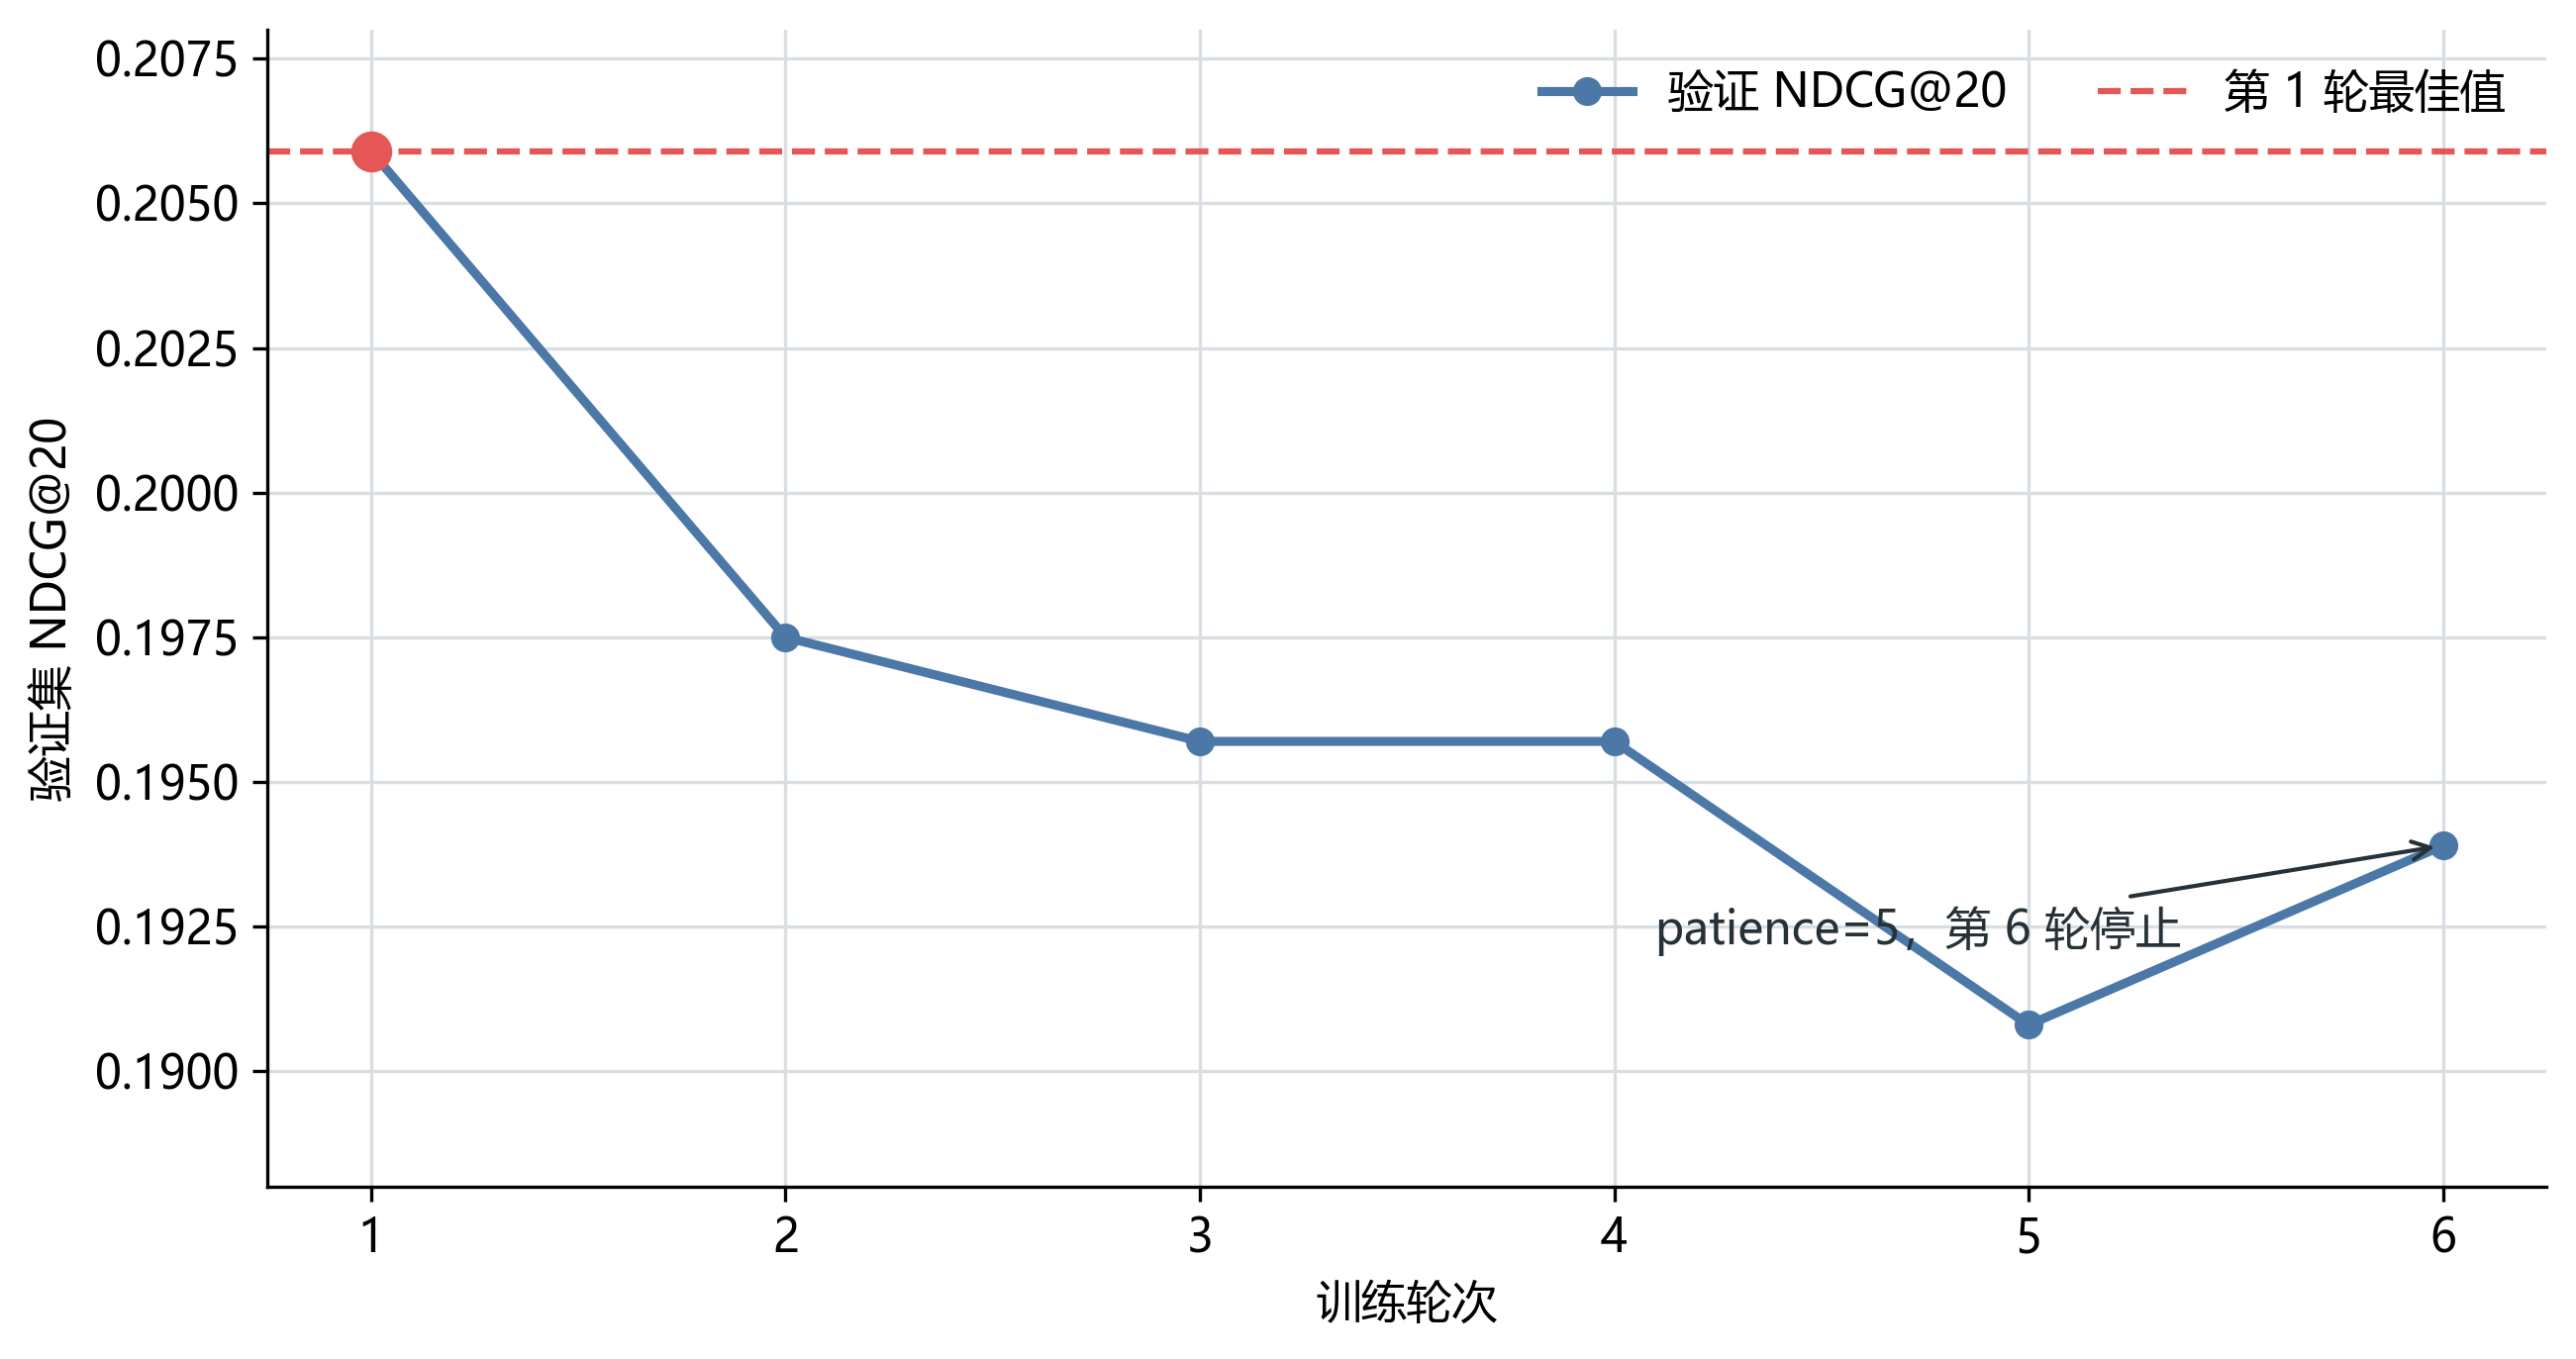
\includegraphics[width=0.82\textwidth]{fig3_early_stop_curve.png}
  \caption{MovieLens-1M 上 SimGCL 连续重跑的验证曲线。最佳轮次后连续 5 轮未提升，于第 6 轮终止。}
  \label{fig:early-stop}
\end{figure}

\section{实验结果与分析}

\subsection{资源受限子集结果}

\begin{table}[H]
  \centering
  \caption{资源受限子集测试结果}
  \label{tab:pilot-results}
  \small
  \begin{tabular}{llrrrr}
    \toprule
    数据集 & 模型 & HR@10 & NDCG@10 & HR@20 & NDCG@20\\
    \midrule
    Grocery\_Pilot & BPRMF & 0.0840 & 0.0389 & 0.1880 & 0.0645\\
    Grocery\_Pilot & LightGCN & \textbf{0.1260} & \textbf{0.0586} & \textbf{0.2120} & \textbf{0.0801}\\
    Grocery\_Pilot & SimGCL（调优） & 0.0960 & 0.0471 & 0.1740 & 0.0665\\
    \midrule
    ML\_1M\_Pilot & BPRMF & 0.4106 & \textbf{0.2205} & \textbf{0.6166} & \textbf{0.2720}\\
    ML\_1M\_Pilot & LightGCN & \textbf{0.4158} & 0.2159 & 0.6075 & 0.2641\\
    ML\_1M\_Pilot & SimGCL（调优） & 0.1244 & 0.0518 & 0.2370 & 0.0800\\
    \bottomrule
  \end{tabular}
\end{table}

Grocery 子集上，LightGCN 四项指标均最高，说明图传播即使在较小数据上也能利用协同关系。SimGCL 把 $\lambda$ 从 0.2 降至 0.01 后，NDCG@20 从 0.0485 提升到 0.0665，提升约 37.1\%，并略高于 BPRMF 的 0.0645。这表明小规模、短训练条件下对比损失权重非常敏感，过强的均匀性约束可能干扰推荐主任务。

MovieLens 子集只有 100 名用户，而 InfoNCE 的批内负例正是其他用户或物品。用户数量过少会降低对比负例的多样性，再加上最多 10 轮和较小嵌入维度，使 SimGCL 明显落后。该现象主要说明资源受限子集不适合验证论文中的最终性能结论，但可以用于发现实现错误和观察超参数行为。

\subsection{完整数据结果}

\begin{table}[H]
  \centering
  \caption{完整数据测试结果}
  \label{tab:full-results}
  \small
  \begin{tabular}{llrrrr}
    \toprule
    数据集 & 模型 & HR@10 & NDCG@10 & HR@20 & NDCG@20\\
    \midrule
    Grocery & BPRMF & 0.3007 & 0.1467 & 0.3990 & 0.1716\\
    Grocery & LightGCN & \textbf{0.3065} & 0.1467 & \textbf{0.4186} & 0.1750\\
    Grocery & SimGCL & 0.2773 & \textbf{0.1761} & 0.3896 & \textbf{0.2042}\\
    \midrule
    MovieLens-1M & BPRMF & 0.4814 & 0.2689 & 0.6785 & 0.3188\\
    MovieLens-1M & LightGCN & \textbf{0.4908} & \textbf{0.2766} & \textbf{0.6952} & \textbf{0.3284}\\
    MovieLens-1M & SimGCL & 0.2781 & 0.1551 & 0.4140 & 0.1893\\
    \bottomrule
  \end{tabular}
\end{table}

\begin{figure}[H]
  \centering
  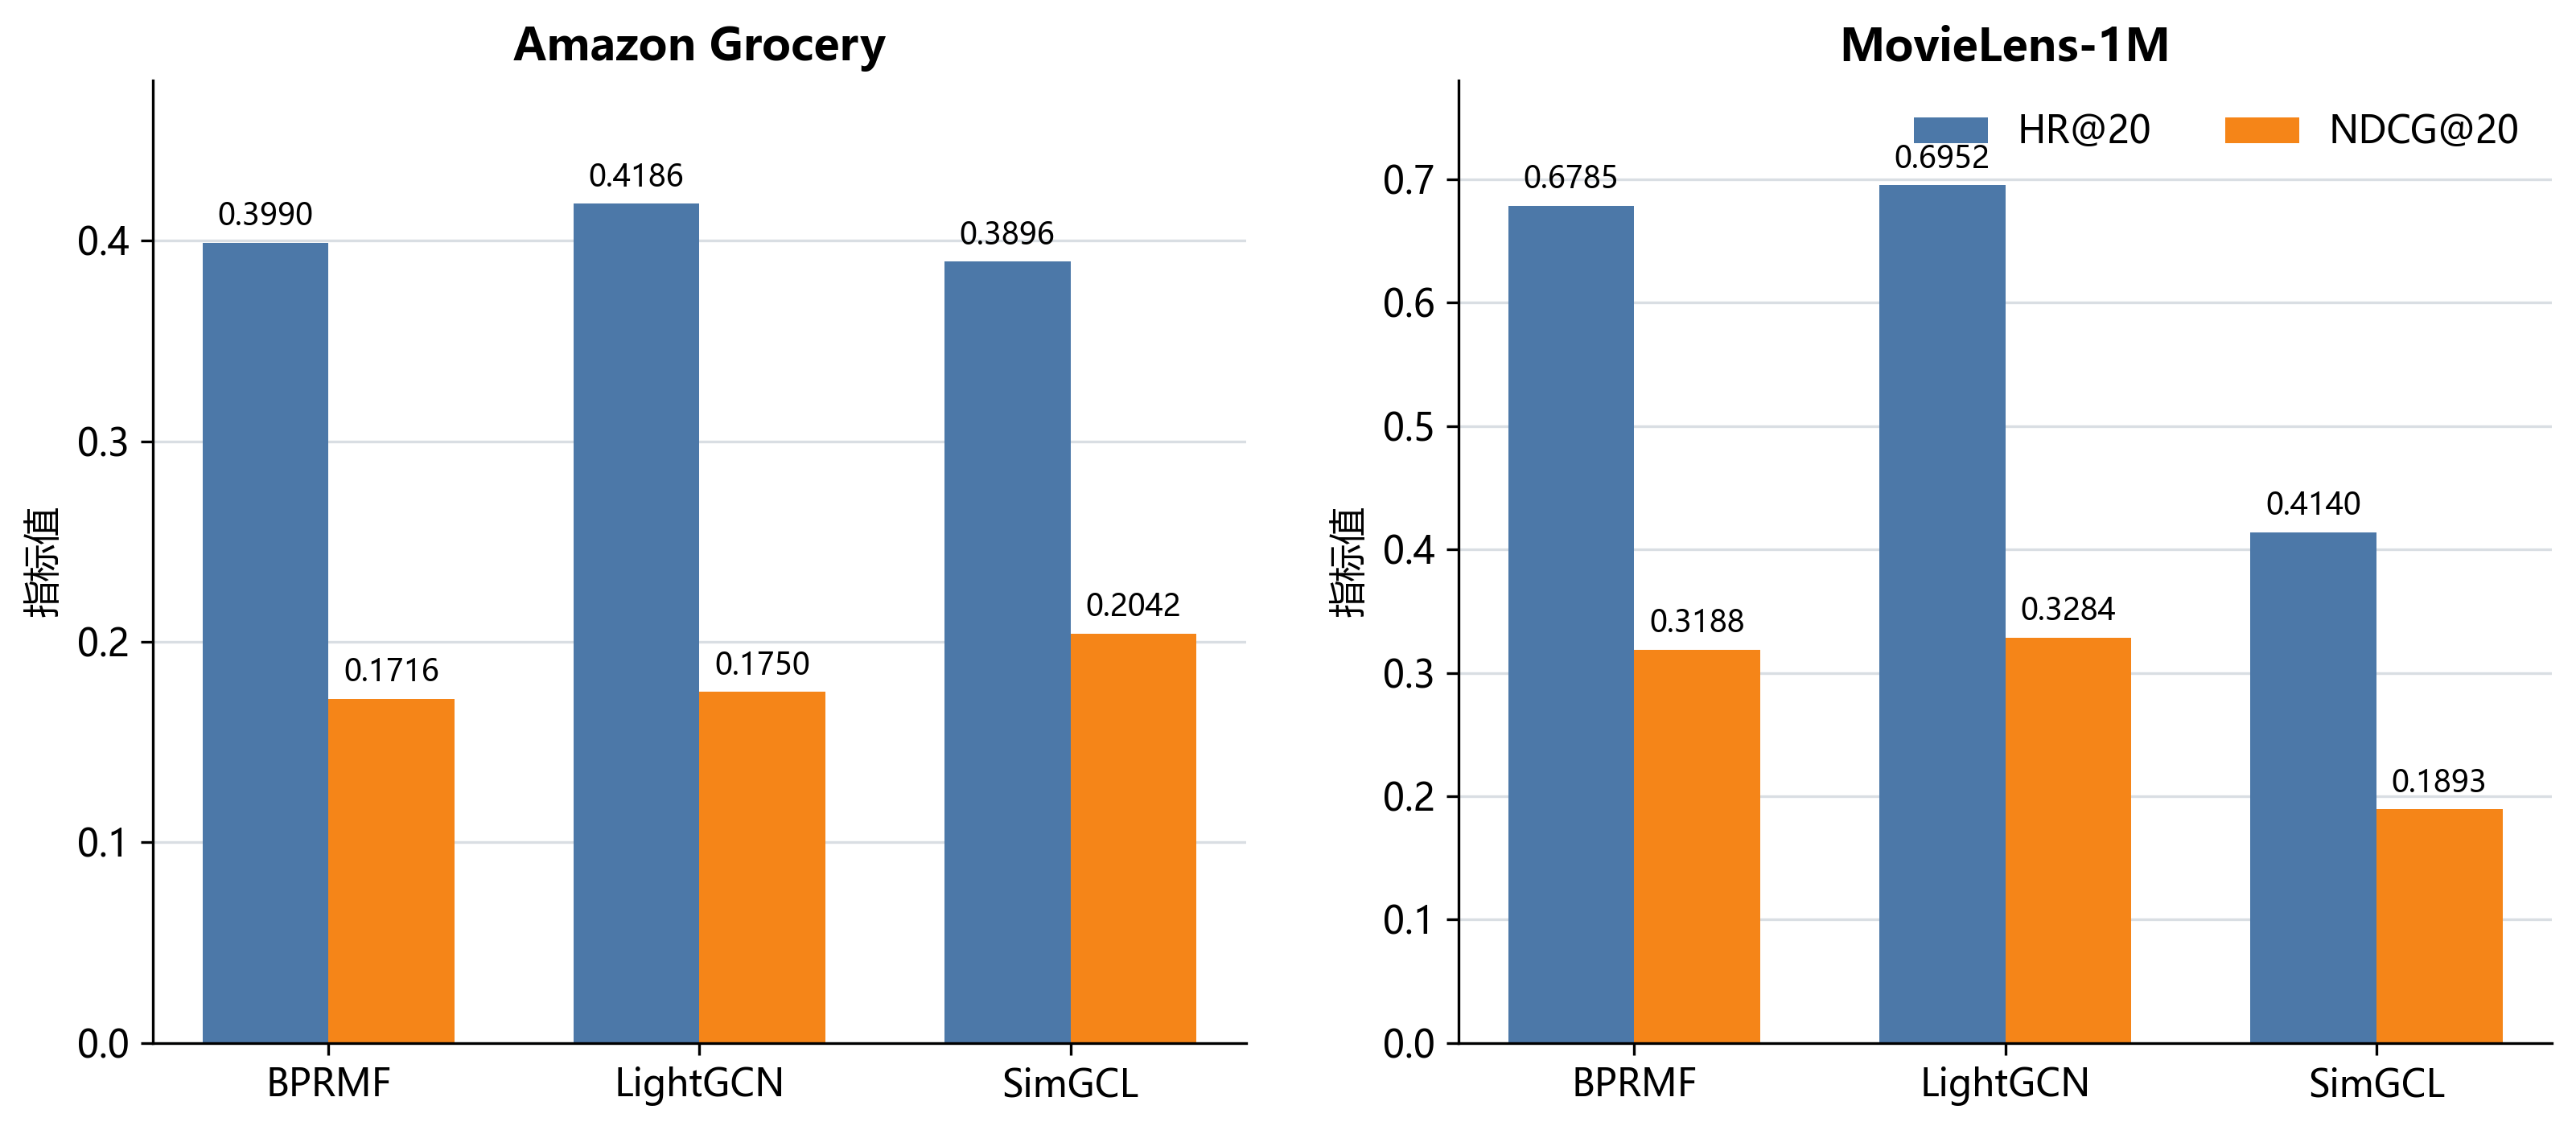
\includegraphics[width=0.98\textwidth]{fig4_full_results.png}
  \caption{完整数据上的 HR@20 与 NDCG@20 对比（1 个正例加 99 个负例）。}
  \label{fig:full-results}
\end{figure}

Grocery 完整数据上，SimGCL 的 NDCG@20 为 0.2042，相比 LightGCN 的 0.1750 提升约 16.7\%，相比 BPRMF 的 0.1716 提升约 19.0\%。然而其 HR@20 为 0.3896，低于 LightGCN 的 0.4186。这意味着在当前配置下，SimGCL 没有命中更多正物品，但能把已命中的正物品排到更靠前的位置。该结果符合 InfoNCE 改善表示分布与排序质量的直觉，但也反映了准确率目标和排序位置目标并不总是同步变化。

MovieLens-1M 上，LightGCN 的四项指标均最高，BPRMF 次之，SimGCL 明显落后。连续重跑后的 SimGCL 测试 NDCG@20 为 0.1893，而 LightGCN 为 0.3284。可能原因包括：固定 $\lambda=0.2$ 未经过完整验证集搜索；ReChorus 的候选采样协议与原论文全物品排序不同；MovieLens 时间划分具有明显分布漂移；以及只运行一个随机种子。由于三个模型在本数据集上使用相同输入和评价候选，框架内比较仍然有效，但不能将差异简单解释为 SimGCL 理论无效。

\subsection{运行与早停情况}

\begin{table}[H]
  \centering
  \caption{完整实验最佳轮次与停止轮次}
  \label{tab:epochs}
  \begin{tabular}{llrrl}
    \toprule
    数据集 & 模型 & 最佳轮次 & 停止轮次 & patience\\
    \midrule
    Grocery & BPRMF & 23 & 32 & 10（历史运行）\\
    Grocery & LightGCN & 25 & 34 & 10（历史运行）\\
    Grocery & SimGCL & 30 & 34 & 5\\
    MovieLens-1M & BPRMF & 1 & 6 & 5\\
    MovieLens-1M & LightGCN & 1 & 6 & 5\\
    MovieLens-1M & SimGCL & 1 & 6 & 5\\
    \bottomrule
  \end{tabular}
\end{table}

规范日志累计训练时间为 10,160.5 秒，即约 2.822 小时，其中包含保留下来的历史尝试。MovieLens SimGCL 连续重跑耗时约 5,842 秒，是 CPU 环境中最耗时的一组。

\section{正确性验证与工程改进}

本项目不仅检查程序能否运行，还对公式与实验结果进行可审计验证：

\begin{itemize}
  \item 验证单层噪声差向量的 L2 长度等于 $\epsilon$，并且与传播表示位于同一超象限；
  \item 验证两次扰动视图不同，推理阶段不构造对比视图；
  \item 用显式矩阵公式复算 InfoNCE，并与模型函数输出比较；
  \item 验证批内重复用户和物品只参与一次对比；
  \item 验证 SimGCL 与 LightGCN 在 CPU 上能够完成前向、反向和有限梯度更新；
  \item 验证 MovieLens 的时间划分、ID 重映射以及负例与已交互集合不相交；
  \item 验证累计预算跨日志生效；
  \item 验证完整续跑状态能够恢复模型、Adam、验证历史与随机数状态；
  \item 独立启动只评估进程加载正式 SimGCL 检查点，复算结果与汇总 CSV 完全一致。
\end{itemize}

最终共有 10 项自动测试通过。工程上的主要改进包括：完成 SimGCL 的 ReChorus 原生接入；修复 LightGCN 的硬编码 CUDA；建立确定性数据脚本；将试验、调参和最终汇总分离；增加累计时间限制；保存完整断点状态；保留旧结果以支持审计；并统一 CPU/GPU 脚本的 patience=5。

\section{局限性与进一步工作}

本实验已经满足课程要求的“两个数据集、两个以上同类基线、统一框架对比”，但与论文级严格复现仍有差距：

\begin{enumerate}
  \item 只使用随机种子 2026，没有按 SimGCL 原论文重复 5 次并报告均值和标准差；
  \item 采用 99 负例采样评价，而原论文采用全物品排序；
  \item 完整数据只使用固定 $\lambda=0.2$，未在完整验证集上搜索 $\lambda$、$\epsilon$ 与层数；
  \item Grocery 两个早期基线使用 patience=10，其余使用 patience=5。虽然日志显示保留的最佳轮次不受后续等待影响，但协议并非形式上完全一致；
  \item CPU 稀疏运算存在轻微非确定性。同一随机种子的两次第一轮验证 HR@20 相差约 0.0019，但 NDCG@20 相同；
  \item 尚未进行长尾物品分组、表示均匀性和流行度偏差分析。
\end{enumerate}

后续若获得 CUDA 环境，应优先进行完整验证集网格搜索，并用 3--5 个随机种子重复全部模型；同时切换到全物品排序，补充均匀性指标、长尾 Recall/NDCG 和显著性检验。这样才能更接近 SimGCL 原论文的实验结论。

\section{结论}

本文完成了 SimGCL 在 ReChorus 中的实现，并在 Amazon Grocery 与 MovieLens-1M 上同 BPRMF、LightGCN 进行了完整比较。实现遵循论文的逐层噪声、同超象限约束、跳过第 0 层、批内 InfoNCE 与 BPR 联合优化。完整实验表明，SimGCL 在 Grocery 上取得最高 NDCG@20，说明对比学习能够改善命中物品的排序位置；但在 MovieLens-1M 上，未经完整数据调参的固定配置明显落后于两个基线，反映了方法对数据划分和损失权重的敏感性。

实验过程中发现，只有模型权重的中断续跑不足以保证优化轨迹连续。通过从零重跑、独立检查点评估和完整状态恢复测试，最终结果的可信度得到提高。综上，本项目已形成一套可运行、可复核、可继续扩展的课程实验实现，但其结论应限定在当前 ReChorus 数据与候选采样协议内，不应被表述为对原论文全排序结果的完全复刻。

\section*{小组分工}
\addcontentsline{toc}{section}{小组分工}



\begin{table}[H]
  \centering
  \begin{tabularx}{\textwidth}{lX}
    \toprule
    成员 & 主要工作 \\
    \midrule
    \underline{鲁越} & 论文阅读、模型实现、实验运行 \\
    \underline{何天佑} & 结果分析、报告整理 \\
    \bottomrule
  \end{tabularx}
\end{table}

\appendix
\section{复现实验命令}

在 \path{ReChorus} 目录安装依赖并运行测试：
\begin{verbatim}
pip install -r requirements-experiment.txt
python -m unittest discover -s tests -p "test_*.py" -v
\end{verbatim}

运行完整 CPU 实验：
\begin{verbatim}
python experiments/run_full_cpu.py --time-limit-hours 10 \
  --epochs 200 --patience 5 --runs-per-invocation 1 --seed 2026
\end{verbatim}

若有 CUDA 环境，可运行：
\begin{verbatim}
powershell -ExecutionPolicy Bypass -File experiments/run_full_gpu.ps1
\end{verbatim}

关键产物为：
\begin{itemize}
  \item \path{experiments/results_full_cpu/results.csv}：完整结果；
  \item \path{experiments/results_full_cpu/status.json}：累计状态；
  \item \path{experiments/results_full_cpu/logs}：权威训练日志；
  \item \path{experiments/results_full_cpu/models}：最佳模型；
  \item \path{experiments/results_full_cpu/interrupted}：旧中断结果归档。
\end{itemize}

\begin{thebibliography}{99}

\bibitem{simgcl}
J. Yu, H. Yin, X. Xia, T. Chen, L. Cui, and Q. V. H. Nguyen.
\newblock Are Graph Augmentations Necessary? Simple Graph Contrastive Learning for Recommendation.
\newblock In \emph{Proceedings of SIGIR}, 2022, pp. 1294--1303.

\bibitem{rechorus}
王晨阳, 任一, 马为之, 张敏, 刘奕群, 马少平.
\newblock ReChorus：一个综合、高效、易扩展的轻量级推荐算法框架.
\newblock \emph{软件学报}, 2022, 33(4): 1422--1440.

\bibitem{lightgcn}
X. He, K. Deng, X. Wang, Y. Li, Y. Zhang, and M. Wang.
\newblock LightGCN: Simplifying and Powering Graph Convolution Network for Recommendation.
\newblock In \emph{Proceedings of SIGIR}, 2020, pp. 639--648.

\bibitem{bpr}
S. Rendle, C. Freudenthaler, Z. Gantner, and L. Schmidt-Thieme.
\newblock BPR: Bayesian Personalized Ranking from Implicit Feedback.
\newblock In \emph{Proceedings of UAI}, 2009, pp. 452--461.

\bibitem{infonce}
A. van den Oord, Y. Li, and O. Vinyals.
\newblock Representation Learning with Contrastive Predictive Coding.
\newblock arXiv:1807.03748, 2018.

\bibitem{rechorus2}
J. Li, H. Li, Z. He, W. Ma, P. Sun, M. Zhang, and S. Ma.
\newblock ReChorus2.0: A Modular and Task-Flexible Recommendation Library.
\newblock In \emph{Proceedings of RecSys}, 2024, pp. 454--464.

\end{thebibliography}

\end{document}
